
\section{Introduction}
\begin{frame}
  \frametitle{Context}
  \begin{columns}
    \begin{column}{0.45\textwidth}
      \begin{block}{Neutron}
        \begin{itemize}
          \item Neutral particle
          \item Wave–particle duality
          \item Magnetic moment
        \end{itemize}
      \end{block}
    \end{column}
    \begin{column}{0.45\textwidth}
      \begin{block}{As probe}
        \begin{itemize}
          \item High penetration
          \item Large scale
          \item 
        \end{itemize}
      \end{block}
    \end{column}
  \end{columns}
  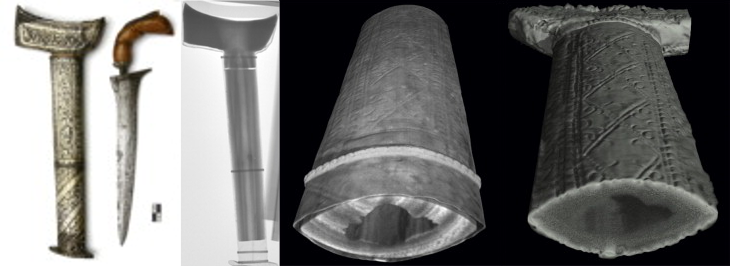
\includegraphics[width=\textwidth]{01_Neutron/fig/fig000_Dague.png}
\end{frame}

\subsection{Context}
\begin{frame}
  \frametitle{State of Neutron sources}
  \begin{block}{Producing neutron}
    Producing neutron is not a trivial task
  \end{block}
  \begin{columns}
    \begin{column}{0.45\textwidth}
      \begin{block}{Fission reactor}
        Use fission reaction:
        \begin{equation*}
          _{92}^{235}U + n \rightarrow X + Y + k \times n
        \end{equation*}
        Continuous flux
      \end{block}
    \end{column}
    \begin{column}{0.45\textwidth}
      \begin{block}{Accelerator Driven Source}
        Two methods:
        \begin{itemize}
          \item
          \item Spallation: with dense target ()
        \end{itemize}
        The properties of theses sources strongly depends on the accelerator.
      \end{block}
    \end{column}
  \end{columns}
  \begin{block}{Spallation}
    Spallation is efficient : a single particle/target collision can generate more than 20 neutrons ...
  \end{block}
\end{frame}

\begin{frame}
  \frametitle{State of Neutron sources}
  \begin{columns}
    \begin{column}{0.50\textwidth}
      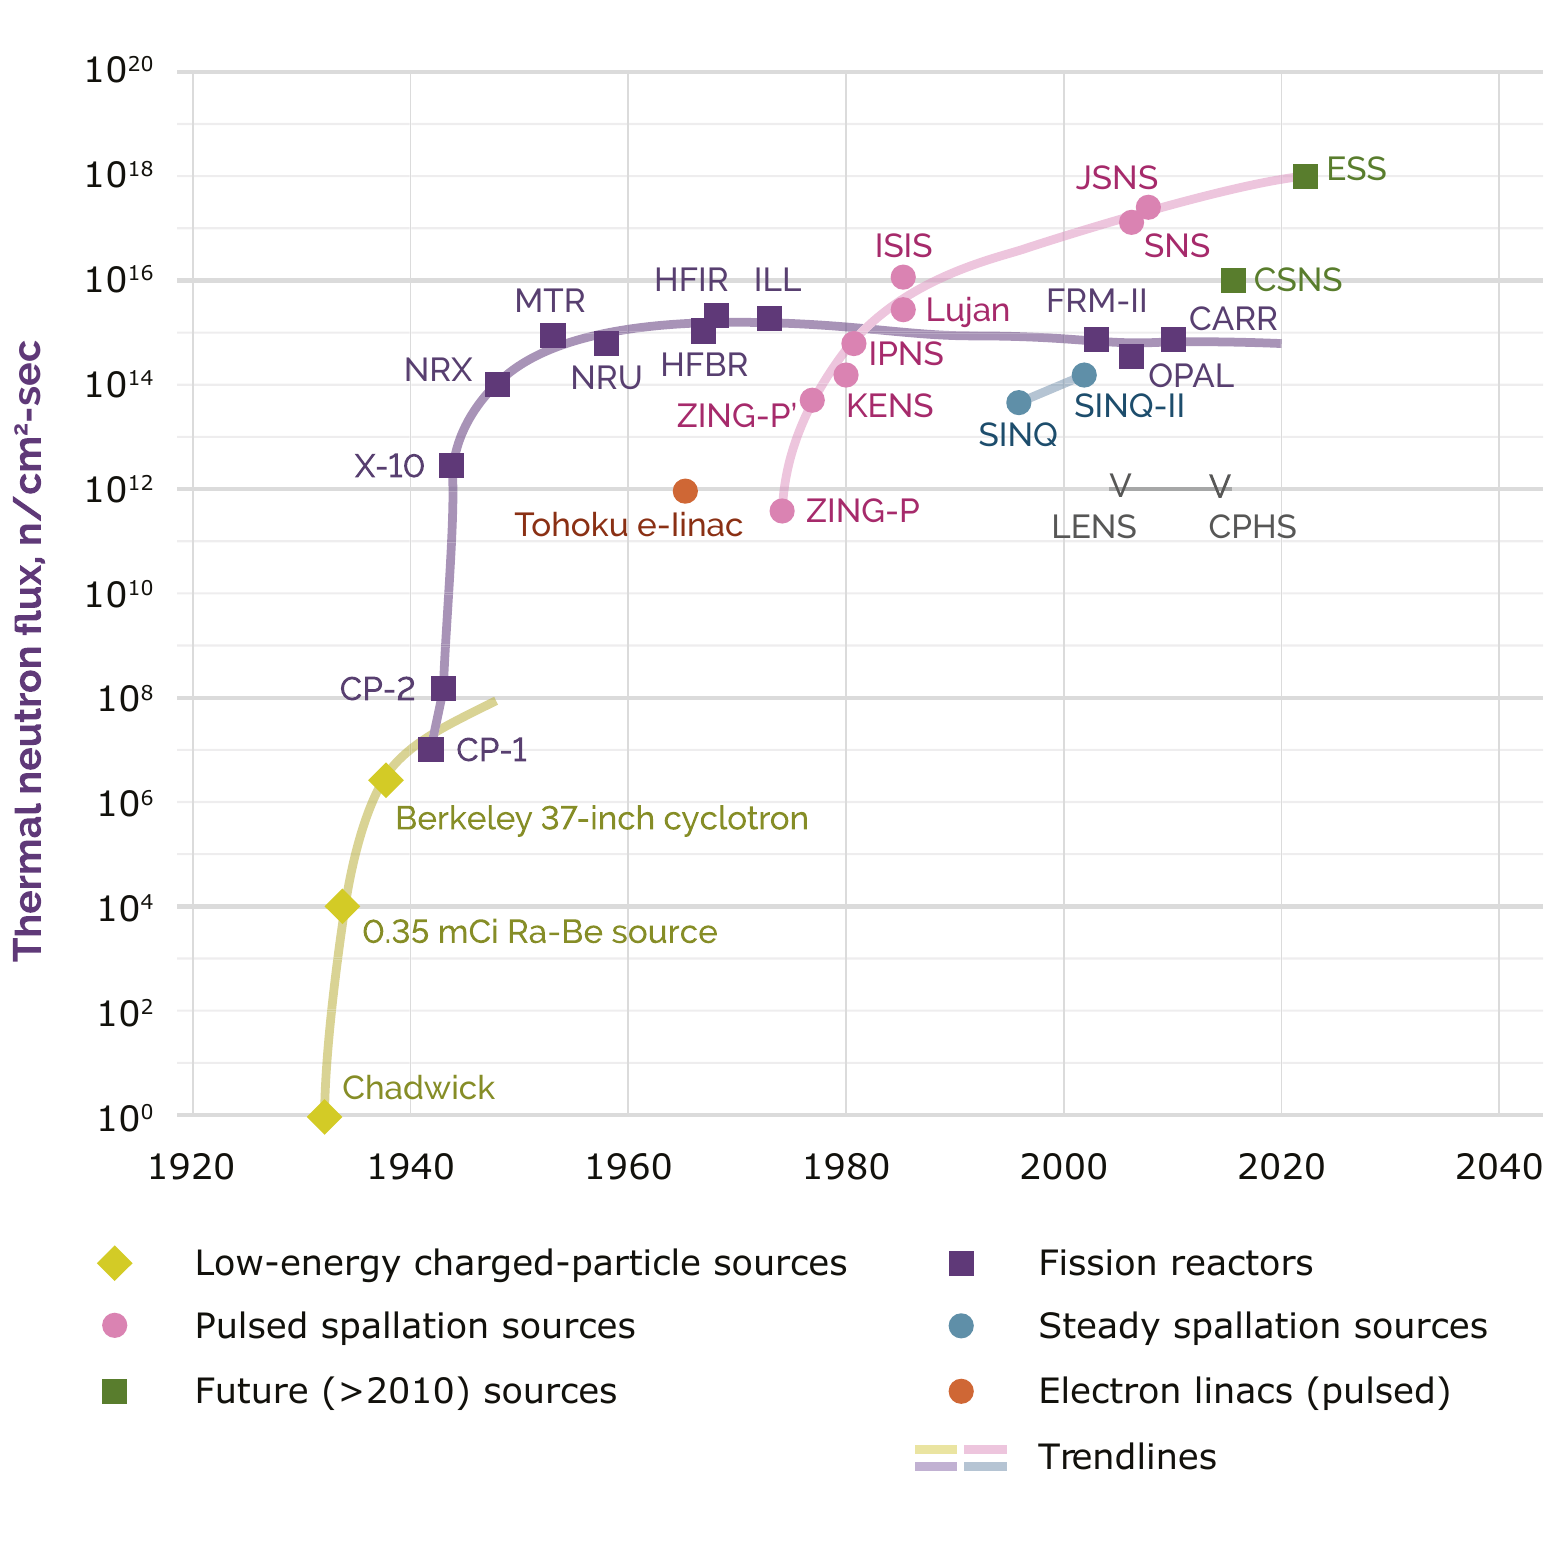
\includegraphics[width=\textwidth]{01_Neutron/fig/fig000_NeutronSources_a}
    \end{column}
    \begin{column}{0.50\textwidth}
      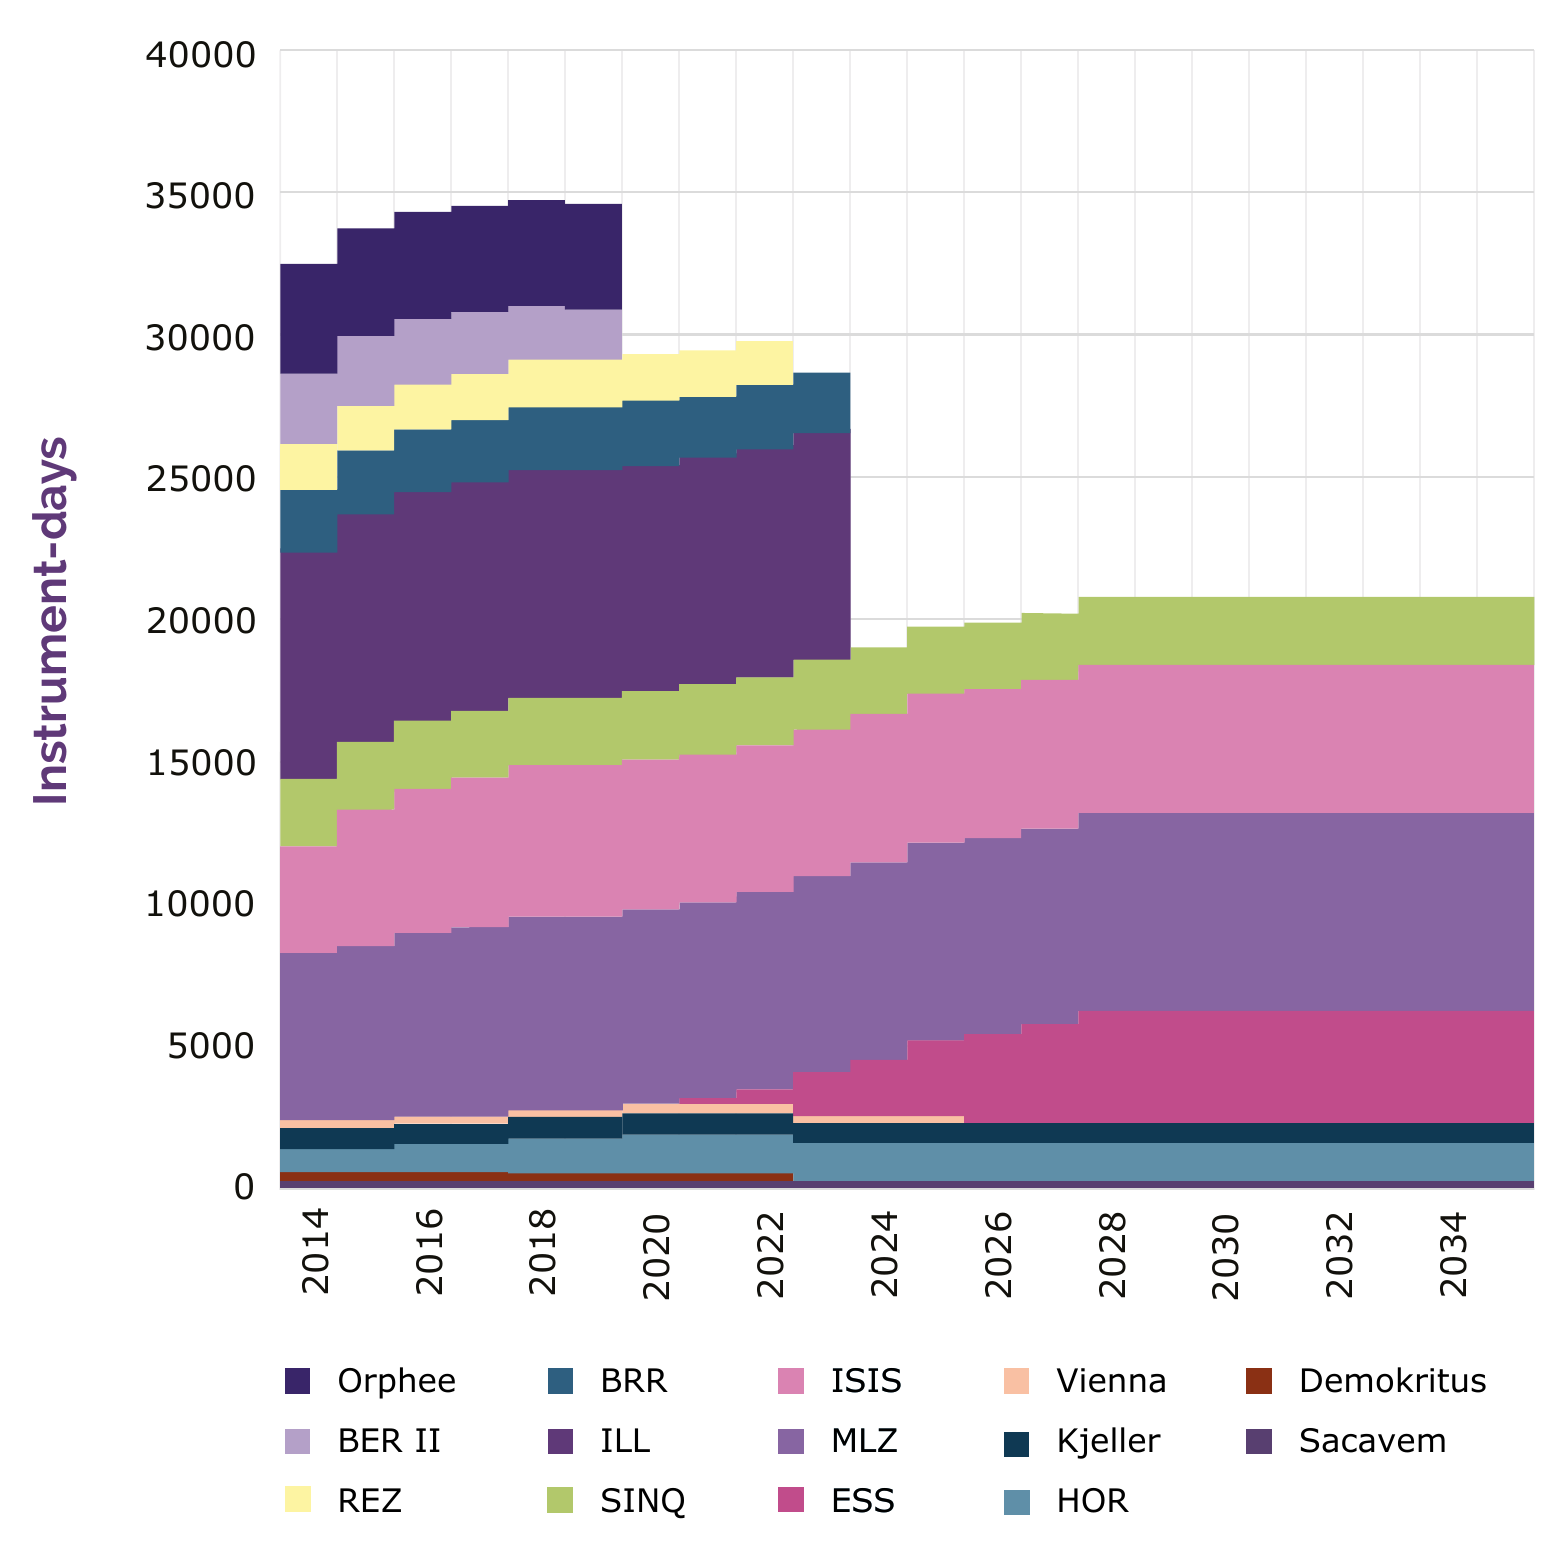
\includegraphics[width=\textwidth]{01_Neutron/fig/fig000_NeutronSources_b}
    \end{column}
  \end{columns}
  From "Neutron scattering facilities in Europe" report by ESFRI
\end{frame}

\subsection{European Spallation Source}
\begin{frame}
  \frametitle{European Spallation Source}
  \begin{block}{Mandate}
    ESS will be the next high end European neutron source.

    Based on a 2 GeV proton accelerator and a tungsten target
  \end{block}
  \begin{columns}
    \begin{column}{0.4\textwidth}
      \begin{block}{Key points}
        \begin{itemize}
          \item[2014] Ground breacking
          \item[2021] First protons on target
          \item[2023] Beginning of user program
          \item 15 neutron instruments
          \item Total cost: 1.8 B€
        \end{itemize}
      \end{block}
    \end{column}
    \begin{column}{0.65\textwidth}
      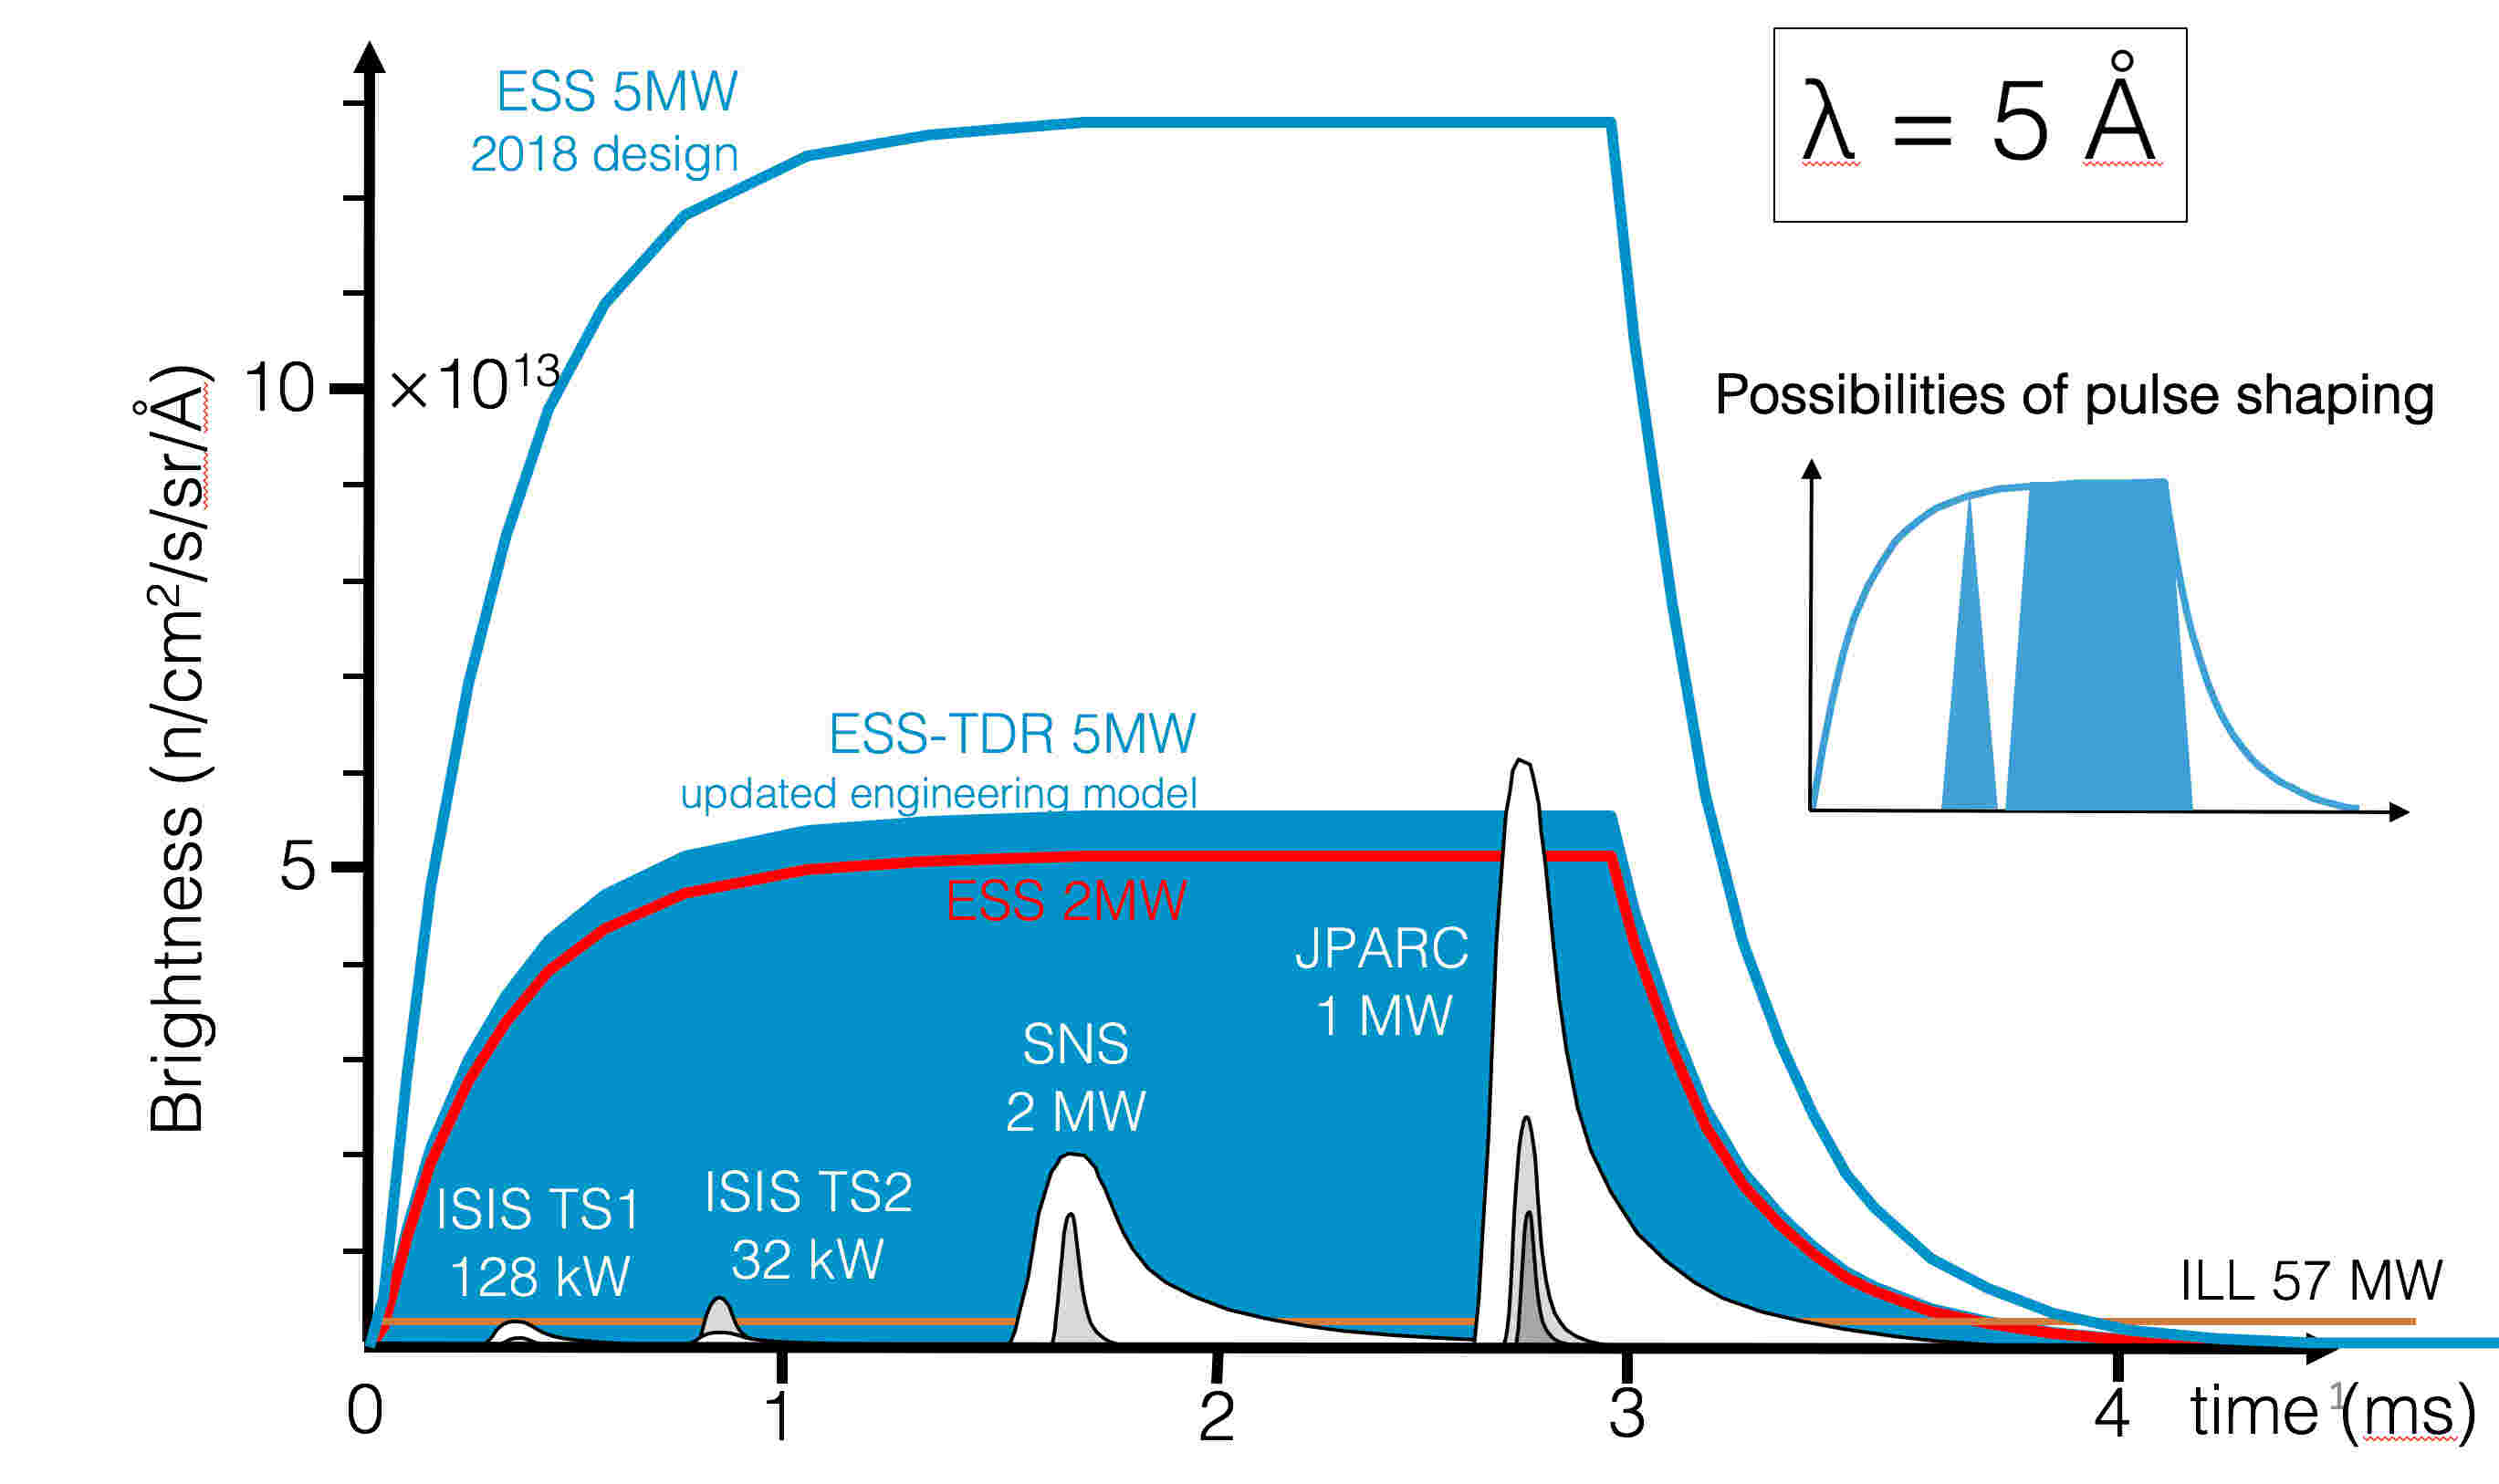
\includegraphics[width=\textwidth]{01_Neutron/fig/fig000_ESS_pulse.jpeg}
    \end{column}
  \end{columns}
\end{frame}

\begin{frame}
  \frametitle{The accelerator}
  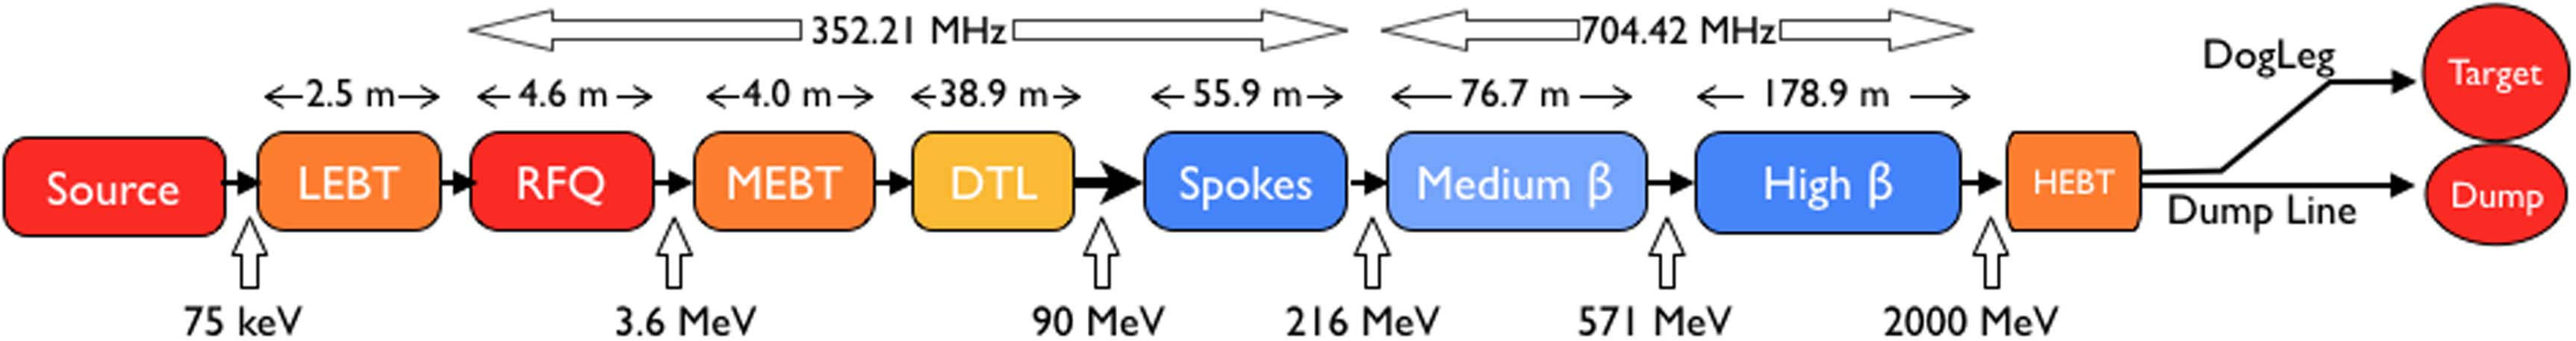
\includegraphics[width=\textwidth]{01_Neutron/fig/fig000_ESS_acc}
  \vfill
  \begin{columns}
    \begin{column}{0.45\textwidth}
      \begin{block}{Key points}
        The accelerator itself is a big challenge.
        \begin{itemize}
          \item 600 m long with 356 m of acceleration
          \item d
          \item 95.5
        \end{itemize}
      \end{block}
    \end{column}
    \begin{column}{0.50\textwidth}
      \begin{tabularx}{\linewidth}{XX}
        \toprule
        Characteristic & Value                                 \\
        \midrule
        Energy         & $2\,\mathrm{GeV}$                     \\
        Current        & $62.5\,\mathrm{mA}$                   \\
        Duration       & $2.86\,\mathrm{ms}$                   \\
        Rep. rate      & $14\,\mathrm{Hz}$                     \\
        Duty cycle     & $4\,\mathrm{\%}$                      \\
        Power (peak)   & $5\,\mathrm{MW}$ ($125\,\mathrm{MW}$) \\
        RF             & $352.21\,\mathrm{MHz}$                \\
                       & $704.42\,\mathrm{MHz}$                \\
        \bottomrule
      \end{tabularx}
    \end{column}
  \end{columns}
\end{frame}